%%% This LaTeX source document can be used as the basis for your technical
%%% report. Intentionally stripped and simplified
%%% and commands should be adjusted for your particular paper - title, 
%%% author, citations, equations, etc.
% % Citations/references are in report.bib 

\documentclass[conference,backref=page]{acmsiggraph}
\usepackage{url}

\TOGonlineid{45678}
\TOGvolume{0}
\TOGnumber{0}
\TOGarticleDOI{1111111.2222222}
\TOGprojectURL{}
\TOGvideoURL{}
\TOGdataURL{}
\TOGcodeURL{}

% Include this so that citations show up in blue and the page information is included in the reference section
\hypersetup{
	colorlinks = true, 
	linkcolor = blue,
	anchorcolor = red,
	citecolor = blue, 
	filecolor = red, 
}


\title{Simulation of a Cloth-Like Structure in a Dynamic 3D Environment\\
	Design Document}

\author{Beej Persson \thanks{e-mail:40183743@live.napier.ac.uk} \\
	Edinburgh Napier University\\
	Physics-Based Animation (SET09119)}
\pdfauthor{Beej Persson}

\keywords{physics-based, animation, simulation, cloth, forces, rigid body, collisions, mesh, springs}

\begin{document}
	
	\teaser{
		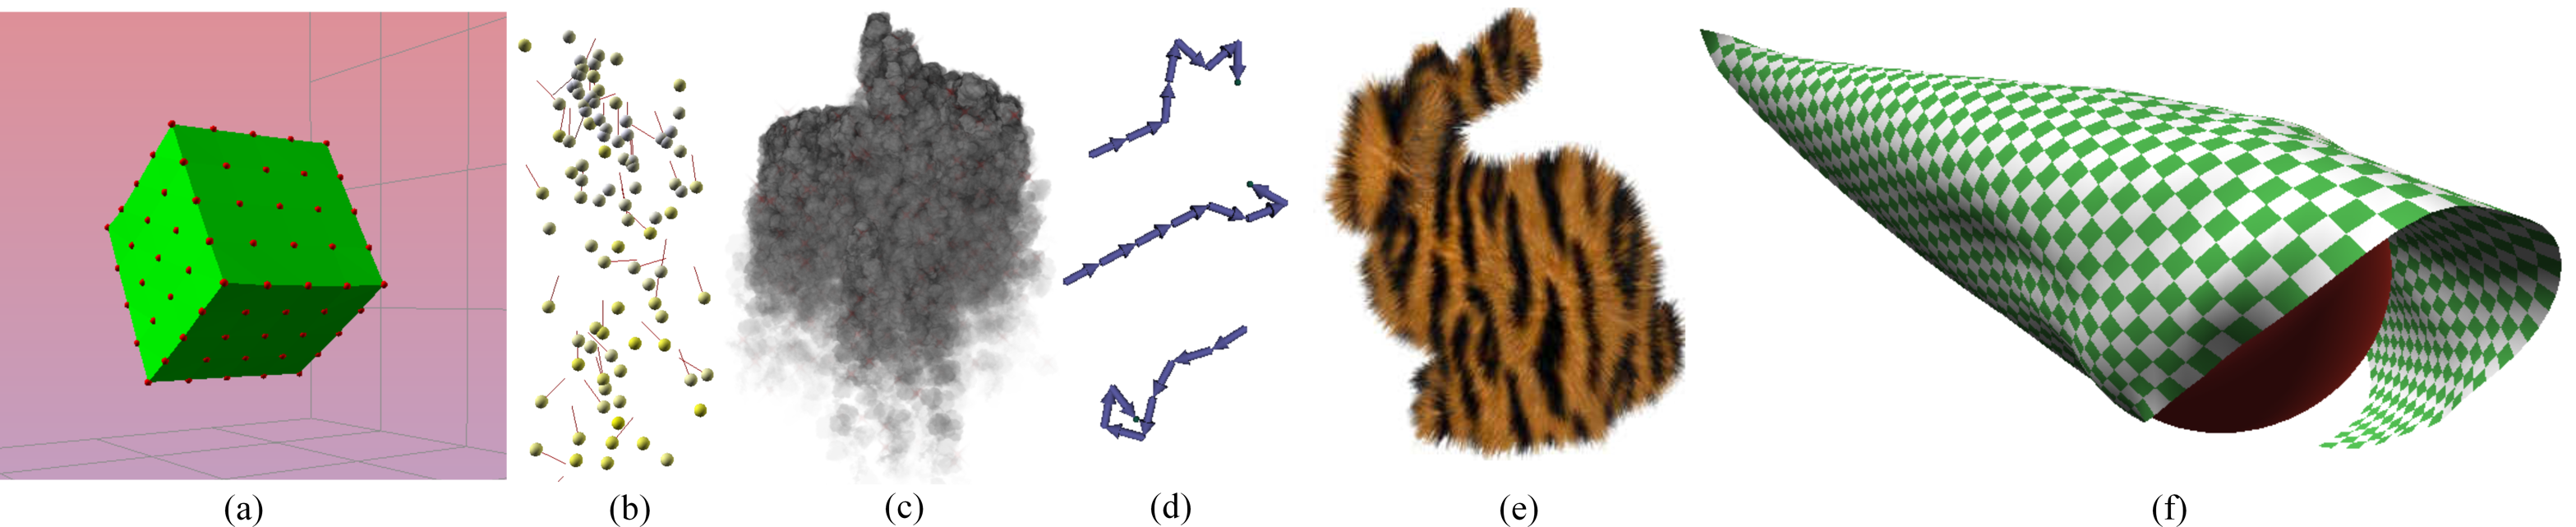
\includegraphics[height=1.5in]{images/sampleteaser}
		\caption{(a) A vortex applied to a sail, (b) cloth made up from a mesh of interconnected springs, (c) flag simulation, (d) rigid body and cloth collision simulations.}
		\label{teaser}
	}
	
	\maketitle
	
	\raggedbottom
	
	\begin{abstract}
		
		This document looks to outline the design of the proposed simulation idea, providing a blueprint that will be used to reflect on the success of the later implementation. The core idea of the intended design for this idea is to simulate a directional force being applied to a cloth-like structure. The desired final aesthetic will be an interactive leaf-blower directed towards either a curtain attached to a curtain rail, a ships sail or a flag, or a choice of the above. The simulation should also include the option to throw small objects at the cloth structure or drape the cloth over certain objects and see its effects. (The images in Figure \ref{teaser} are (a) \cite{sail}, (b) \cite{clothmesh}, (c) \cite{flag} and (d) \cite{object}.)
		
	\end{abstract}
	
	
	
	\keywordlist
	
	%% Use this only if you're preparing a technical paper to be published in the 
	%% ACM 'Transactions on Graphics' journal.
	
	% \TOGlinkslist
	
	% \copyrightspace
	
	
	\section{Introduction}
	
	
	%notes
	
	\paragraph{What problem are you solving?}
	Physically simulating natural looking cloth-like structures has often been one of the harder aspects in games, especially if interaction with the cloth is required (a character walking through drapes in a doorway, or sheets on a washing line). For the most part they are simply animated to move in a way such that it looks as though it is reacting to its environment, effected by the wind or a characters motion, when in fact it isn't. This is in part due to the difficulty of accurately simulating cloth physics without significantly affecting performance. This project will attempt to deal with these problems.
	
	
	\paragraph{What is the motivation?}
	If cloth physics can be accurately simulated, 3D game environments can take a significant step in the direction of realism and immersion. With the Virtual Reality industry expanding as fast as it is any increase in immersion is highly desired.
	
	\paragraph{Challenge \& Limitations}
	Simulating the physics of cloths can be a very difficult process due to the "incredibly complex interactions that cloth has on the macro and microscopic levels" \cite{kristopher}. There are three main approaches to simulating cloths, geometric, physical and particle based techniques, and each has their own issues. Geometric basic techniques work well for single-frame renders but not for dynamic models \cite{Weil}. Physical methods are better at dynamically modelling cloth but still don't take into account micro-interactions happening within the cloth \cite{Feynman}. Finally, particle based modelling better accounts for the complex interactions happening withing the interior of cloth structures but is the most taxing on performance \cite{Breen}.
	
	\paragraph{Our Work}
	The intended technique to be used in this proposed simulation idea is to model the cloth as a system of interconnected particles, following the work of David Breen and a tutorial based off of what he's done. This may be limited by the amount of time available for the project, and simple techniques may need to be explored instead.
	
	\paragraph{Starting Examples}
	This design document attempts to highlight the current difficulties associated with simulating cloth-like structures in a 3D environment by considering the limitations of the methodologies discussed and in doing so indicate how the proposed simulation idea addresses these limitations.
	
	
	\section{Related Work}
	The most famous initial piece of work on cloth physics was Weil's geometric approach \cite{Weil} in which he represented the cloth as a grid of multiple points. Weil's work forms the basis for almost all other cloth simulation techniques \cite{Karthikeyan}. Feynman in 1986 also modelled the cloth using a grid, but using Equation \ref{eq:physical} below:
	
	\begin{equation} \label{eq:physical}
		E(Particle_{i,j}) = k_{s}E_{s,i,j} + k_{b}E_{b,i,j} + k_{g}E_{g,i,j}
	\end{equation}
	
	Where $s$ is Elasticity, $b$ is its bendiness and $g$ its density, Feynman observed that the final shape of the cloth is created when the energy of the cloth is at a minimum. Thus creating a way for modelling cloths that accounted for a materials stretch, stiffness and weight. David Breen, one of the foremost people who has worked in modelling cloths using particle systems, has attempted many different forms of the particle based modelling technique over the years. A general approach to the particle model is to suppose that there is a network of particles interacting with each other and by modelling the properties of this micro-structure and their interactions a realistic motion in the cloth is simulated. This is shown by Equation \ref{eq:particle} below:
	
	\begin{equation} \label{eq:particle}
		U_{Total} = U_{Repel} + U_{Stretch} + U_{Bend} + U_{Trellis} + U_{Gravity}
	\end{equation}
	
	Where $U$ is the energy of the respective elements of the system.
	
	% SIMULATION
	\section{Simulation}
	
	\paragraph{Overview}
	The core principles of the proposed simulation ideas is a system involving a curtain reacting realistically to wind or compressed air from a leaf blower, or similar. Mechanically an interactive object that will be applying a constant and direct force will be pointed towards a cloth-like structure with locked top-nodes to simulate a curtain blowing in the wind.
	
	\paragraph{Detailed description}
	\begin{itemize}
		\item {\bf Functionality}: The simulation will see the effects of a direct force on a cloth, and attempt to animate a realistic reaction to this force (refer to (a) in Figure \ref{teaser}). For the possible additions of different cloth structures, the functionality will be similar (with a directional force applied to the flag or sail), but the reaction should be different due to differing locked nodes. There may also be the ability to drape a cloth over an object and have objects thrown at the different cloths.
		\item {\bf Method}: The primary equation when dealing with the force applied to the cloth and its reaction will be Equation \ref{eq:fma} shown below:
		
		\begin{equation} \label{eq:fma}
			F = m\cdot a
		\end{equation}
		
		Where $F$ is the force, $m$ the mass and $a$ the acceleration. The three techniques, as described above, for modelling cloths are Geometric, physical and particle based models.
		
		\item {\bf Control/interactivity}: The leaf blower will be moveable and the power and size of the cone of force should be manipulatable, allowing differing intensities of force to be applied to different sections of the cloth.
	\end{itemize}
	
	\paragraph{Implementation}
	
	\begin{itemize}
		\item  {\bf Major Software Development Tasks} The primary difficulty will be accurately simulating the motion of the cloth when impacted by the force. Developing the cloth physics will likely be difficult to implement. Other important tasks are to simulate the specific type of force a leaf blower applies.
		\item {\bf Risks} If particle based modelling of the cloth-like structure proves too difficult or time consuming simpler models may need to be used to complete the project.
	\end{itemize}
	
	% EVALUATION
	\section{Testing and evaluation}
	Certain tests will be carried out to ensure that the simulation works within the desired environment. For example, testing whether or not the cloth reacts realistically to the effect being hit by a thrown object or draped over a sphere. Tests will be run to analyse the performance of the software and whether its inefficient or too taxing on the GPU. Tests with volunteers will be run to determine if the design of the interactivity is intuitive and easy to use.
	
	
	\section{Conclusion and Future work}
	The desired design of the proposed simulation idea is to see the effects of focused air on a cloth-like structure with certain nodes locked in place (for example the top nodes for the rail of a curtain). There are three main modelling approaches: geometric, physical and particle based systems. The intended method to be used is a particle based model where the cloth's micro-structure is modelled by having a network of particles interacting with each other and determining the desired position of each particle (and therefore shape of the cloth) by using the energy Equation \ref{eq:particle} show above. There are certain challenges that will need to be overcome, and tests will be run to evaluate the effectiveness of the desired simulation.
	
	
	% \section*{Acknowledgements}
	
	
	\bibliographystyle{acmsiggraph}
	\bibliography{report}
	
\end{document}